\section{Different types of controllers}
The control input in a feedback system is the value that tells the system under control to behave slightly different than it did and possibly incorporating external disturbances on the system in a better way. As discussed in the previous section, this control input value is computed in the controller part of the feedback system. Although one might expect differently, the controller itself does not turn out to be very smart or know a whole lot about the system under control. As mentioned before, a controller in fact only needs to know about directionality of the system and the magnitude of the correction for it to work just fine. There are a number of controllers that only need these two pieces of information and that are commonly used in physics, mechanics and electronics.

\subsection{On/Off control}
The most simple controller one can think of is just an \textit{on/off switch}. Whenever the tracking error is positive, the controlled system is turned on and when the tracking error becomes negative it is turned off again\footnote{Of course this is dependent upon the directionality of the system under control.}. For simple systems this kind of control will suffice, although it will not be a very effective approach.

An application of this kind of control might be a air conditioning system that turns on when the temperature exceeds a preset level. In this example the control output is the current temperature in the room, the setpoint is the preset temperature, the control input is a boolean value which determines whether the system should be on of off and the directionality of the system is negated. Imagine the temperature initially being much too high, causing the air conditioning to turn on right away. After a certain amount of time the temperature reaches the desired setpoint (the tracking error becomes zero), hence the system will shut down. Shortly after the air conditioning system is shut down, the temperature starts increasing again. This immediately causes a deviation from the setpoint, forcing the air conditioning to turn on again. Soon enough the temperature is low enough again for the system to be turned off, after which the cycle starts all over again. Of course this kind of behavior is very annoying to everyone working in this room, as the air conditioning continuously turns off and on again. Besides that, this behavior costs an unnecessary amount of energy for turning the system on and off, which is not really desirable either.

Obviously this behavior is caused by the controller that dictates to turn off the system whenever the setpoint is met. Due to external disturbances such as whether conditions the feedback system is off track soon again, which causes the controller to decide to turn the controlled system back on.

Small improvements that are often used in these kinds of systems are introducing a dead zone or Schmitt trigger, which causes the system to continue with the same corrective action until a certain threshold or a certain amount of time is exceeded. This prevents the controller from overreacting on sudden and short spikes in the control output. In the case of the air conditioning an addition such as this will cause the controller to not immediately send a `turn off signal' when the setpoint is zero and will not activate the system with the slightest deviation, but instead waits a little longer until a threshold is exceeded before activating or deactivating the system again.

\subsection{Proportional control}
\label{subsec:prop-control}
Another improvement on the on/off controller is to change the output. Rather than sending a boolean value to the controlled system, a real controller should send a floating point value. The \textit{proportional controller} does this by taking the magnitude of the error into account when calculating the magnitude of the corrective action. If the tracking error is small, the control input should be small and if a large tracking error occurs, the control input should be proportionally large. To achieve this, the proportional controller uses the following formula:

\begin{equation} \label{eq:proportional-control}
u_p(t) = k_p \cdot e(t) \text{\ \ \ \ where } k_p > 0 \text{ constant}
\end{equation} 

Here $u_p(t)$ and $e(t)$ are the control input and the tracking error at time $t$ respectively and $k_p$ is the proportional controller gain, which is a positive constant. The control input is thus calculated by multiplying the \emph{current} tracking error with the controller gain, hence the control input is proportional to the tracking error.

In practice this kind of controller in a feedback system has the effect of applying small changes to the control input when the tracking error is small and larger changes for a bigger tracking error. Although this may work just fine for some systems, other system show the same kind of problem as with the on/off controller. For this we need to study the behavior of a proportional controller when the tracking error approaches zero: due to \autoref{eq:proportional-control}, the control input becomes proportionally smaller and eventually becomes zero at the moment the tracking error becomes zero. At this point in time the feedback system has reached its desired state and (needless to say) has to keep the control output there as close as possible. However, the tracking error is zero and hence the control input is zero. For systems like the air conditioning this is equivalent to turning itself off. As with the on/off controller, turning off the air conditioning causes the temperature to rise again due to the external disturbances on the system. With that the tracking error becomes non-zero again and gives rise to the controller to turn the system back on, to only get the tracking error back to zero and turning off the air conditioning.

Although the proportional controller is a slight improvement in regard to the on/off controller in the way it translates the tracking error into the next control input as well as in the more fine-tuned way of representing this control input, it still shows the problem of not working correctly in the case of approaching the setpoint value. This problem will however be fixed in a later section.

\subsection{Integral control}
A third way of coming up with the next control input that is quite common in feedback control is to not only look at the current tracking error, but also at all the previous tracking errors. \textit{Integral control} does this by using the running sum of both the current and all previous tracking errors. As is well known from mathematics, in a continuous stream a sum becomes an integral (hence the name), resulting in \autoref{eq:integral-control-continuous}.

\begin{equation}\label{eq:integral-control-continuous}
u_i(t) = k_i \int_{0}^{t}e(\tau) \mathrm{d} \tau \text{\ \ \ \ where } k_i > 0 \text{ constant}
\end{equation}

Here $u_i(t)$ and $e(\tau)$ are the control input and the tracking error at times $t$ and $\tau$ respectively and $k_i$ is the integral controller gain, which is a positive constant.

Although \autoref{eq:integral-control-continuous} is useful for continuous systems that occur in physics and engineering, it does not apply to computer science as in that field everything is discrete. Therefore \autoref{eq:integral-control-discrete} will be used instead, which is mathematically the discrete counterpart of the integral.

\begin{equation}\label{eq:integral-control-discrete}
u_i(t) = k_i \sum_{0}^{t}e(\tau) \text{\ \ \ \ where } k_i > 0 \text{ constant}
\end{equation}

All by itself the integral controller is not very useful, as the results (tracking errors) of all previous iterations of the control loop are still incorporated in the same proportion as the result from the current iteration. In his book, Janert \cite{janert2013-feedback} briefly shows a very simple toy example for this controller working all by itself, but here no external forces are applied on the system and the model is fully known. A further exploration of this use case is described in a blog post ``\textit{Feedback Control for Hackers}'' \cite{heest2015-feedback-for-hackers}. In most situations the integral controller is however not practically usable by its own. However, as we will see in section~\ref{subsec:combining-controllers}, combining it with other types of controllers creates a very powerful tool that will turn out very effective.

\subsection{Derivative control}
The proportional controller and the integral controller in the previous sections respectively took the present and the past values for the tracking error into account when coming up with the next control input. The basis for the latter is founded in the mathematical concepts of integrating the tracking error. It should therefore not come as a surprise that another kind of controller can be created that tries to predict the future values for the tracking error and takes these predictions into account when calculating the next control input. This is done by calculating the derivative of the tracking error signal and using that as a way to predict the next tracking errors. From mathematics it is well-known that if the derivative of a signal is positive, the value of the signal is currently growing (and vice versa). This can be applied to the tracking error signal, from which actions can be taken to bring the signal closer to the desired value.

Mathematically we can express the derivative controller by the following equation:

\begin{equation}\label{eq:derivative-control}
u_d(t) = k_d \frac{\mathrm{d} e(t)}{\mathrm{d} t} \text{\ \ \ \ where } k_i > 0 \text{ constant}
\end{equation}

Here $u_d(t)$ and $e(t)$ are the control input and the tracking error at time $t$ respectively and $k_d$ is the derivative controller gain, which is a positive constant.

Although predicting the future sounds promising, Janert \cite{janert2013-feedback} points to a number of problems with the derivative controller. First of all, sudden changes in the setpoint will momentarily cause very large spikes in the output of the derivative controller (a.k.a. the control input), which are sent to the system under control. This effect is also known as \textit{derivative kick}. On the other hand, many systems produce a control output signal that is full of high-frequency noise. Taking the derivative of such a signal will cause an enhancement of the effect of the noise. For this reason it is often a necessity to smooth the signal, which in itself brings both extra complexity and the risk of defeating the purpose of having derivative control with it, as over-smoothing the signal will eliminate exactly those variations that the derivative controller was supposed to pick up.

\subsection{Combining controllers}
\label{subsec:combining-controllers}
So far we have discussed four types of controllers, of which one calculates a boolean value and the others calculate a floating point number. All of these controllers by them selves turned out to have various problems that caused them to be unusable individually in a feedback control system. One of the most prominent problems is caused by the proportional controller not working correctly when approaching the setpoint. This is due to the fact that the control input approaches zero as the tracking error approaches zero.

This problem is often solved by combining the proportional controller with the integral controller. Here the tracking error is sent to both the proportional and integral controller after which their outputs are combined by addition. This newly composed controller is often referred to as a \textit{PI controller}. The integral term of this controller takes care of the problem by providing a nonzero contact offset, such that when the proportional term approaches zero, the integral term will still be there and cause the PI controller to produce a nonzero output.

When the air conditioning system is controlled by a feedback loop with a PI controller, it will try to bring the temperature to the desired value and with that make the tracking error as small as possible. When the desired temperature is reached the system will \emph{not} turn off, but rather keeps running, presumably on a low enough setting such that the temperature stays the same. When an external disturbance causes the temperature to rise, the tracking error becomes nonzero again, which makes the proportional controller more active again and makes both components of the PI controller contribute to bringing the temperature back to the desired level.

Another combination of controllers is referred to as a PID controller. This combines the powers of the proportional, integral and derivative controller, such that this controller can take present, past and future into account when coming up with the next value for the control input. A common representation of the PID controller is shown in \autoref{fig:pid}. Here it is clearly visible that all three components receive the same tracking error signal, after which all three controllers produce their own output, which eventually get combined by addition into the controller output and control input.

\begin{figure}[H]
	\begin{center}
		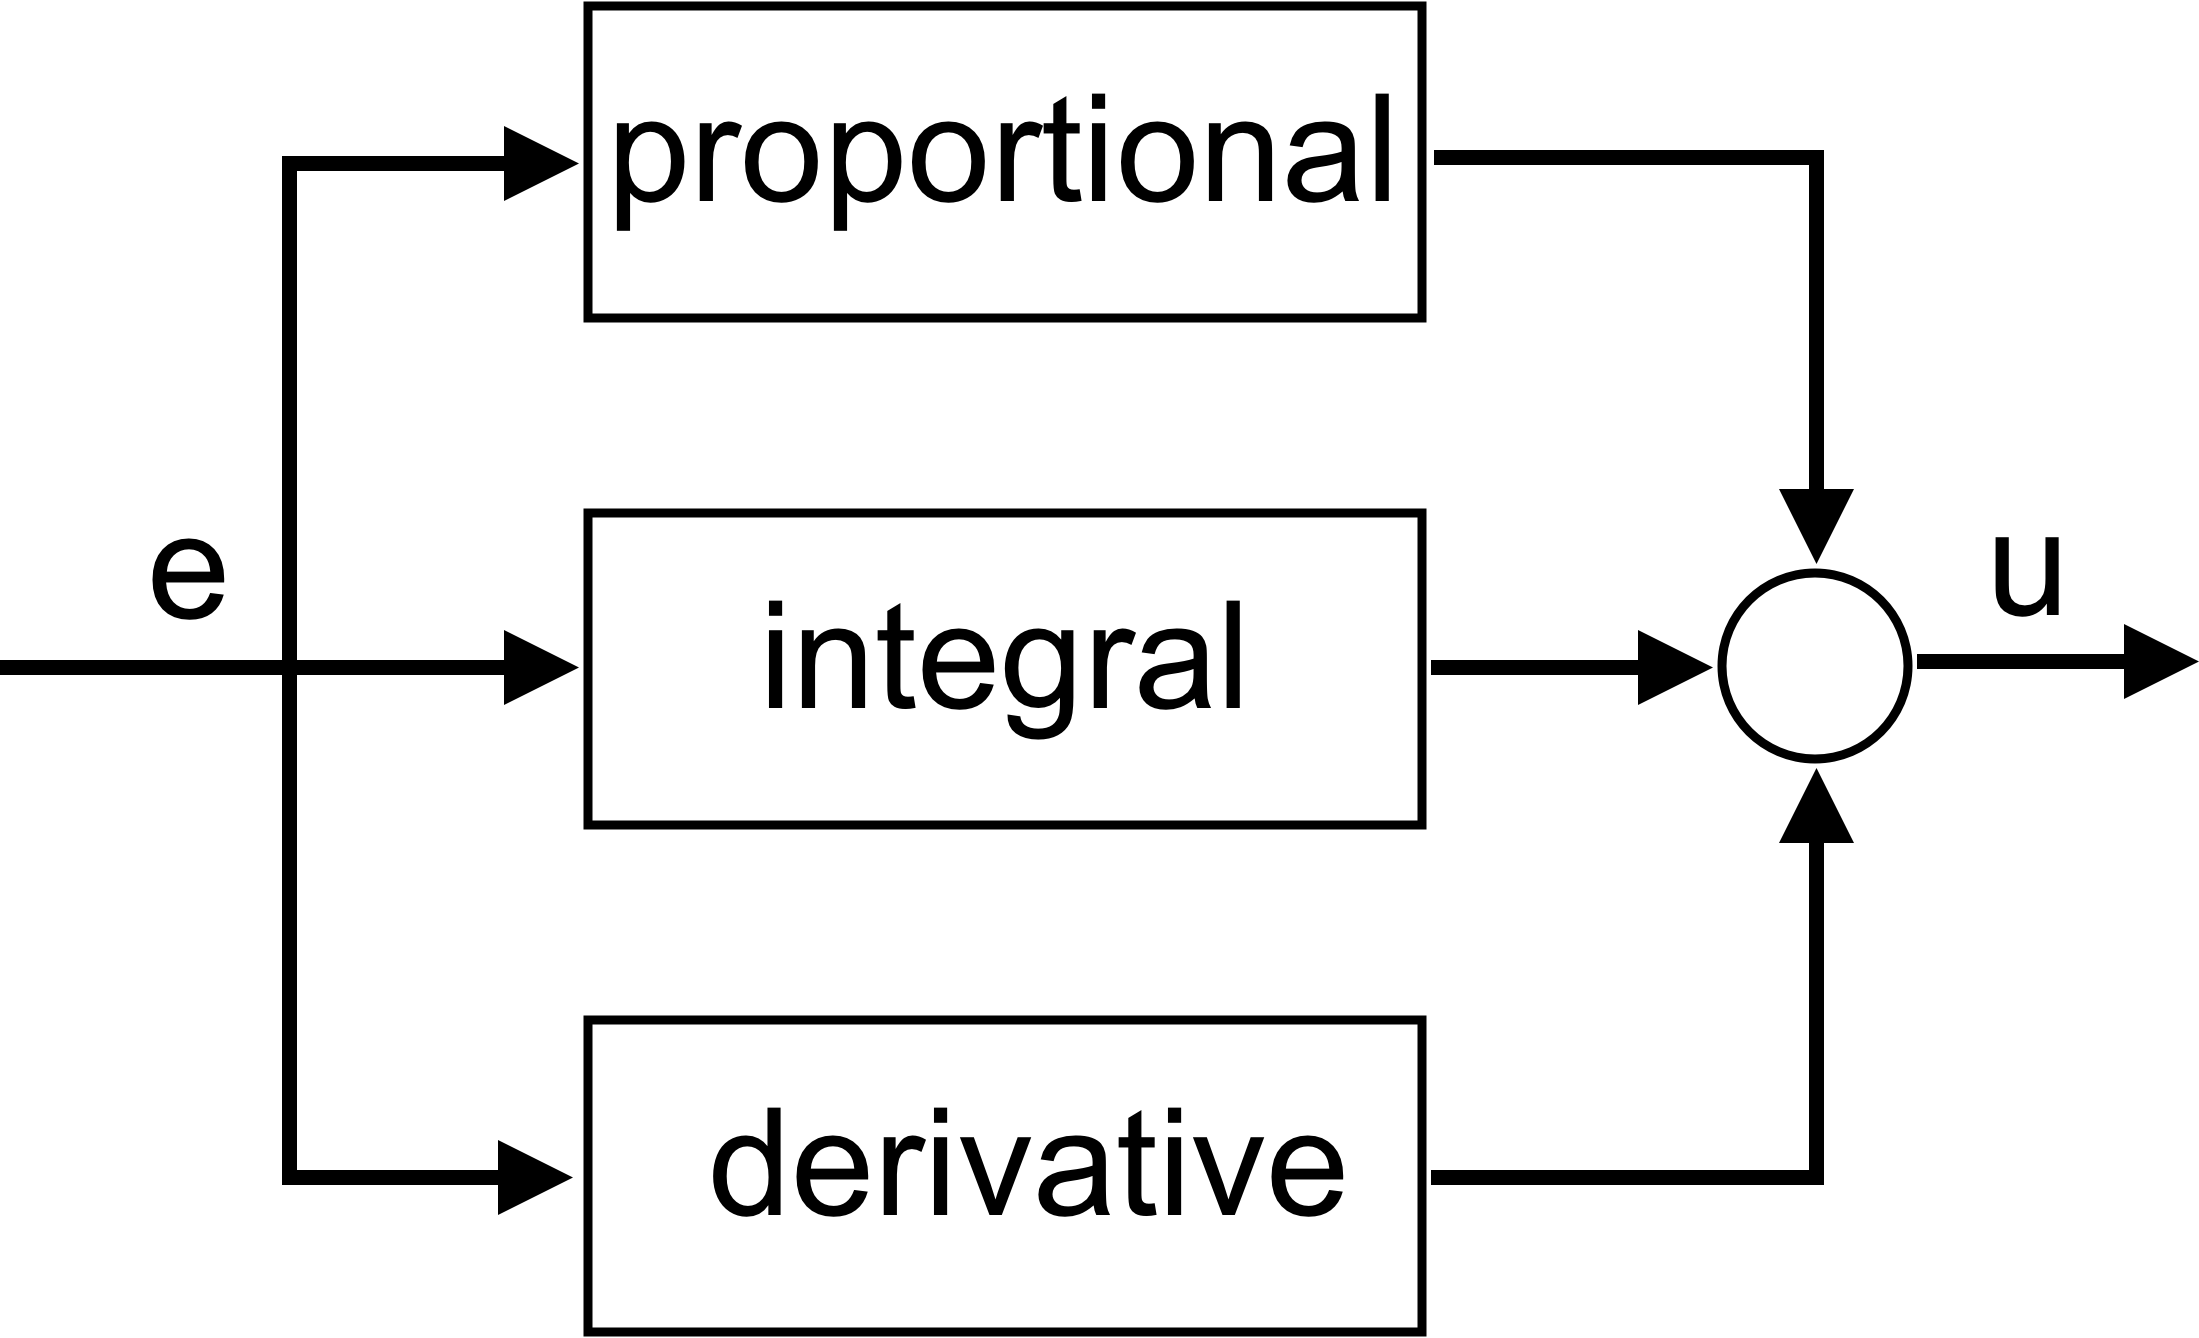
\includegraphics[width=0.60\textwidth]{figures/pid.png}
	\end{center}
	\caption{Combining proportional, integral and derivative control}
	\label{fig:pid}
\end{figure}

A drawback to these composed controllers concerns the controller gains that are involved in each part of the controller. With the PID controller we have to come up with three separate values that each determine the level of involvement of the different components in the whole controller. These three constants together determine how well the whole feedback system is working and a careful choice for these values is therefore crucially important! The topic of controller tuning will however be considered outside the scope of this thesis. Regarding this topic we refer to both Hellerstein et al. and Janert \cite{hellerstein2004-feedback, janert2013-feedback} for extended and in-dept discussions. Also the blog post ``\textit{Feedback Control for Hackers}'' \cite{heest2015-feedback-for-hackers} discusses this topic by doing a real-world case study based on the work of Janert.
